%versi 2 (8-10-2016)
\chapter{Landasan Teori}
\label{chap:teori}

\section{Pelaksanaan Ujian}
    Pelaksanaan ujian dimulai dengan memperhatikan standar prosedur (SOP) ujian
    di lab\cite{lab:buku-sop}. Standar prosedur ini dibuat oleh Kepala Lab yang
    kemudian diikuti oleh beberpa pihak. Pembahasan pedoman pelaksanaan ujian
    ini akan dimulai dengan membahas pedoman untuk peserta ujian, Pengawas,
    Admin Lab, dan dosen koordinator.
    
\subsection{Pedoman Pelaksanaan Ujian untuk Peserta Ujian}
    Pedoman pelaksaan ujian untuk peserta dimulai beberapa hari sebelum ujian
    dimulai. Peserta diharuskan memperhatikan pengumuman dan jadwal
    \textit{shift} yand diterbitkan oleh Kepala Lab Komputasi (KLK). Peserta
    diharuskan untuk segera melaporkan jika jadwal yang diterbitkan memiliki
    masalah dengan jadwal ujian yang dimiliki oleh peserta, paling lambat satu
    hari sebelum masa ujian dimulai. Jika peserta gagal melaporkan masalah yang
    ada sebelum masa ujian dimulai, maka konsekuensinya peserta akan mengikuti
    jadwal ujian yang telah diterbitkan sebelumnya.

    Menjelang ujian, peserta diharuskan mempersiapkan perlengkapan ujian, dan
    datang dua puluh menit sebelum ujian dimulai. Posisi tempat duduk mahasiswa
    akan mengikuti posisi tempat duduk yang diterbitkan oleh Tim Admin Lab.
    Peserta yang akan memasuki wilayah lab diharuskan menunjukan kartu tanda
    mahasiswa (KTM) pada petugas admin dan lab. Setelah masuk ke dalam lab,
    peserta diharuskan menunggu aba-aba dari Pengawas untuk dapat memasuki
    ruangan ujian. Peserta yang akan masuk hanya diperbolehkan membawa peralatan
    ujian yang izinkan saja.

    Setelah peserta memasuki ruang ujian, peserta dipersilahkan untuk mempersiap
    tempat mengerjakan ujian. Persiapan tersebut meliputi melakukan login pada
    komputer yang ditugaskan, membuka perangkat lunak pendukung dan melakukan tes
    cepat terharap perangkat lunak tersebut. Peserta diharapkan untuk melaporkan
    masalah yang terjadi. Peserta diharuskan melakukan pengumpulan jawaban pada
    sistem Oxam ataupun judge ujian. Lembar jawaban berupa fisik akan
    dikumpulkan ke Pengawas ujian. Peserta yang sudah selesai mengerjakan ujian
    diperbolehkan meninggalkan ruangan.

\subsection{Pedoman Pelaksanaan Ujian untuk Pengawas Ujian}
    Pengawas ujian akan memulai persiapan ujian beberapa saat sebelum jadwal ujian
    dimulai. Pengawas diharapkan datang 15 menit sebelum jadwal ujian. Selain
    itu, Pengawas ujian diharuskan untuk mengambil berkas soal ujian di ruang
    tata usaha, jika terdapat soal ujian dalam bentuk fisik.

    Sebelum ujian dimulai, Pengawas melakukan koordinasi dengan Koordinator
    untuk memastikan kebutuhan ujian seperti pembagian soal, kertas buram, kata
    sandi soal, ralat soal, dan sebagainya. Selain itu, Pengawas diharuskan
    untuk memastikan seluruh peserta memiliki berkas ujian. Setiap masalah yang
    ada akan dibantu bersama Tim Admin. Jika dirasa perlu, pengawas dapat
    memberikan penerangan pada peserta atas aturan ujian, folder pengerjaan
    peserta, tempat pengumpulan jawaban dan kebutuhan lainnya. Pengawas dapat
    memulai ujian dengan memulai timer yang terdapat pada layar proyektor.

    Saat ujian berlangsung, pengawas diharuskan untuk mengedarkan daftar hadir
    untuk ditandatangani mahasiswa dan memeriksa KTM. Setiap kendala teknis yang
    terjadi dapat dilaporkan pada Tim Admin. Tim admin akan berada pada ruangan
    pada lima menit pertama. Setelah lima menit tersebut Tim Admin akan berada
    pada ruang admin. 
    
    Ujian akan berakhir pada saat timer di layar telah habis. Pengawas berwenang
    untuk memutuskan solusi yang diambil jika terjadi masalah pada pengumpulan
    jawaban. Jika ujian hanya memiliki satu \textit{shift}, maka Pengawas dapat
    mengijinkan peserta untuk meninggalkan ruangan saat peserta selesai
    mengerjakan atau waktu ujian telah habis. Jika ujian terdiri lebih dari satu
    \textit{shift}, maka Pengawas dilarang untuk mengijikan peserta keluar dari
    ruangan ujian tanpa koordinasi dengan Tim Admin.

    Setelah ujian selesai Pengawas diharuskan untuk mengisi Berita Acara, daftar
    hadir peserta, berkas tertulis (jika ada) lalu dikumpulkan pada ruangan Tata
    Usaha.
    
\subsection{Pedoman Pelaksaan Ujian untuk Admin Lab}
    Pedoman pelaksanaan dimulai dengan persiapan pelaksaaan. Tim Admin yang
    bertugas diharuskan mengikuti jadwal khusus. Jadwal khusus tersebut terdiri
    dari:
    \begin{itemize}
        \item 45 Menit sebelum ujian Tim Admin diharuskan sudah berada di lab.
        \item Maksimal 30 menit sebelum ujian dimulai, berkas ujian yang
            dibutuhkan sudah harus disiapkan. Berkas tersebut termasuk
            \textit{script}, absensi dan posisi tempat duduk ujian. 
        \item 30 Menit sebelum ujia, posisi tempat duduk ditempelkan pada pintu
            utama Lab untuk dapat dilihat oleh peserta.
        \item 20 Menit sebelum ujian dimulai, Admin membuka pintu utama. Admin
            kemudian akan melakukan pengecekkan KTM. Peserta yang tidak memiliki
            KTM atau surat izin sejenis tidak diperbolehkan untuk memasuki
            lobi. \\
            Admin kemudian memindahkan posisi tempat duduk ke dalam lobi.
        \item 5 Menit sebelum ujian, Tim Admin diharuskan mengunci pintu masuk
            utama lab. Peserta yang terlambat tidak dapat diberi izin untuk
            masuk oleh Tim Admin.
        \item Admin menunggu aba-aba dari pengawas untuk mobilisasi peserta
            masuk ke ruang ujian.
        \item Admin menunggu aba-aba dari pengawas untuk memulai timer.
        \item 5 Menit setelah timer dimulai, Tim Admin diharuskan
            \textit{stand-by} di dalam ruangan ujian untuk menangani masalah
            teknis yang mungkin muncul.
        \item Setelah ujian berakhir, Admin memeriksa jawaban yang sudah
            terkumpul. Jika terjadi masalah, Admin diharuskan untuk melaporkan
            ke pengawas ujian. \\
        Lalu jawaban ujian dikirimkan pada dosen mata kuliah yang bersangkutan.
        \item Untuk ujian dengan lebih dari satu \textit{shift}, Admin
            diharuskan untuk memastikan bahwa pintu belakang telah terbuka
            sebelum shift pertama berakhir.
    \end{itemize}

\subsection{Panduan Ujian untuk Dosen Koordinator}
    Panduan Ujian yang harus diikuti oleh Dosen Koordinator dimulai dengan
    melaporkan kebutuhan khusus ujian paling lambat satu minggu sebelum ujian
    tersebut.  Kemudian dosen Koordinator diharuskan menentukan beberapa hal,
    yaitu
    \begin{itemize}
        \item Jenis ujian, yang terdiri dari: 
            \begin{itemize}
                \item \textit{Softcopy}, soal akan didistribusi ke
                    masing-masing komputer.
                \item \textit{Hardcopy}, soal akan dicetak oleh Tata Usaha seperti pada
                    ujian kelas.
                \item Kombinasi \textit{Softcopy} dan \textit{Hardcopy}.
                \item Dengan layanan lain, seperti \textit{Judge}.
            \end{itemize}
        \item Durasi ujian. Disarankan maksimal 110 Menit.
        \item Tipe ujian, yang terdiri dari:
            \begin{itemize}
                \item \textit{Close Book} (Tidak menggunakan berkas bantuan apapun.)
                \item \textit{Open Book} (Hanya diperkenankan dalam bentuk
                    \texttt{hard copy}.)
                \item \textit{Open File} (Menggunakan berkas yang didistribusi
                    pada folder ujian masing-masing peserta.)
                \item Lainnya (dengan layanan seperti Judge, basis data, dan sebagainya.)
                \item Kombinasi.
            \end{itemize}
        \item Nama dan ekstensi berkas pengumpulan. Penamaan berkas mengikuti
            format \texttt{\<prefix\>xxyyy\<postfix\>} dengan detil:
            \begin{itemize}
                \item \texttt{xx} adalah dua dijit tahun angkatan, dan
                \item \texttt{yyy} adalah NPM dari peserta.
            \end{itemize}
            Pengumpulan berkas lebih dari lima disarankan menggunakan zip.

        \item Kata sandi soal jika diperlukan.
    \end{itemize}

    Soal dan informasi tersebut kemudian dilaporkan pada email-email tertentu
    dan Kepala Lab Komputasi paling lambt satu hari sebelum ujian dimulai.

    Pada saat ujian dimulai, Dosen Koordinator menjadi koordinator pengawas
    ujian. Koordinator pengawas berwenang memberikan instruksi saat ujian
    berlangsung, termasuk aba-aba mulai, pemberian kata sandi, waktu habis dan
    sebagainya.

\section{Perangkat Lunak Berbasis Web}
    Seperti pengembangan aplikasi pada \textit{platform} lainnya, terdapat
    banyak cara untuk mengaplikasikan solusi yang dirancang berdasarkan
    kebutuhan dan batasan yang ada. Pada pengembanagan aplikasi web, karena
    aplikasi tidak hanya berjalan pada \textit{server} atau peladen saja, maka
    secara umum pengembang memecah sistem menjadi dua subsistem besar.
    
    Dua subsistem ini mengikuti pola pemrograman \textit{Server-client}, dengan
    aplikasi klien biasanya ditangani oleh \textit{browser} atau peramban. Namun
    dengan berkembangnya teknologi, sistem pada peramban juga mulai berevolusi.
    Oleh karena itu sistem-sistem yang ada harus dirancang dengan baik sesuai
    dengan disiplin sistemnya sendiri.
    
    Secara umum, front-end akan membantu sistem menampilkan data dengan baik
    dengan memanipulasi peramban pengguna. Sedangkan back-end akan membantu
    mengolah data yang sistem front-end berikan.

\subsection{Back-end}
    Back-end atau Backend adalah sebuah subsistem yang melayani program namun
    tidak diakses secara langsung oleh penggunanya, melainkan dengan melalui
    Front-end\cite{oxford:definition-backend}. Pada umumnya Back-end memiliki
    tugas untuk menyimpan data, memproses data, dan memvalidasi data.
    
    Sesuai dengan namanya, sistem back-end hanya akan berjalan pada server dan
    sumber kode yang terdapat pada sistem ini tidak akan ditampilkan pada
    pengguna.

\subsection{Front-end}
    \textit{Front-end} atau \textit{Frontend} adalah sebuah subsistem yang
    melayani pengguna secara langsung\cite{oxford:definition-frontend}.Front-end
    ini memiliki tugas untuk menyajikan data pada pengguna, serta melakukan
    pemanggilan perintah ke \textit{back-end}.
    
    Sesuai dengan namanya, subsistem front-end akan berjalan pada sisi klien
    dari sistem, oleh karena itu kode subsistem ini harus dapat ditransmisikan
    ke peramban pengguna agar sistem dapat berjalan sesuai ekspektasi. Karena
    kode pada subsistem ini dapat dilihat oleh pengguna, maka sistem back-end
    penting untuk melakukan sanitasi data untuk memastikan data yang diberikan
    tidak mengancam kestabilan siklus hidup sistem keseluruhan.

\section{\textit{Library} dan \textit{Framework}}
    \textit{Library} adalah kumpulan fungsi yang dikompilasi bersama dan
    biasanya dibagikan untuk aplikasi gunakan dengan cara pemanggilan tertentu.
    \textit{Library} biasanya digunakan oleh pengembang atau \emph{developer}
    untuk mempermudah manajemen dan melakukan pemanggilan fungsi tertentu pada
    sistem. Pada pengembangan sistem web, \textit{Library} biasanya mengacu pada
    kumpulan fungsi atau modul-modul yang membungkus sekuens tertentu dan fungsi
    khusus yang disediakan oleh peramban (\textit{browser}) untuk pengembang.
    Maka dari itu istilah \textit{Library} sering juga disebut \textit{Package}
    atau \textit{Module} tergantung dari konteks letak dan peranan fungsi
    tersebut\cite{npm-docs:packages-n-modules}\cite{node-docs:CommonJS-modules}.
    
    \textit{Framework} adalah salah satu bentuk abstraksi yang dibuat untuk
    menyediakan layanan yang generik pada pengembang. Selain itu
    \textit{framework} membantu pengembangan dan penerbitan aplikasi menjadi
    lebih mudah dan cepat. Karena bentuk abstraksi tersebut, struktur kode yang
    dibuat menjadi berpola. Dengan adanya bantuan dokumentasi, pengembang
    aplikasi dapat dengan mudah mencari dan memanfaatkan kode \textit{framework}
    tersebut.
    
    Pada pengembangan sistem web, sebuah \textit{framework} biasanya memiliki
    beberapa \textit{package} yang terdiri dari beberapa \textit{library} atau
    bahkan dibuat \textit{library} baru yang telah dibuat generik berdasarkan
    RFC yang disepakati oleh tim pengembang tersebut\cite{reactjs:rfc}. Lalu
    beberapa \textit{package} dibuat terhubung sedemikian rupa sehingga
    \textit{framework} terbentuk dan dapat digunakan oleh para-pengembang.
    
    Kode yang di-\textit{extend} dari \textit{framework} atau \textit{library}
    memiliki sifat yang universal, dapat digunakan-ulang, yang menyediakan
    fungsionalitas-fungsionalitas kecil yang dapat digunakan untuk membuat
    \textit{platform} aplikasi yang lebih besar. Penggunaan-ulang ini membuat
    pengembangan program menjadi lebih terstruktur dan konsisten. Perubahan
    algoritma pada beberapa bagian program akan dapat langsung memperbaharui
    penggunaan algoritma yang sama di berbagai tempat.
    
    Kode program yang sudah melalui beberapa iterasi dan dianggap sudah "tepat"
    oleh pengembang disebut sebagai \textit{mature} atau matang.
    \textit{Framework} yang digunakan pada umumnya sudah dianggap matang
    (\textit{mature}) oleh pengembang sehingga membuat program memiliki
    \textit{bug} yang lebih sedikit.
    
    \textit{Delivery} adalah penerbitan fitur/fungsi ke kode program di wilayah
    peladen yang digunakan oleh pengguna asli (\textit{production server} /
    peladen produksi). Untuk mencapai \textit{delivery} yang cepat, pengembang
    aplikasi normalnya akan menggunakan kode yang sudah terbukti di
    \textit{medan perang} sehingga pada saat tahap pengembangan para pengembang
    dapat lebih fokus untuk mengimplementasi fitur program, dibandingkan dengan
    pengembang harus menyelesaikan \textit{bug-bug} yang seharusnya tidak perlu
    ada.
    
    \textit{Behaviour} adalah sifat yang fitur/fungsi miliki pada saat melakukan
    algoritma tertentu. Secara kontras, pengembang yang tidak menggunakan
    \textit{framework} harus membuat program dari dasar. Masalah yang timbul
    dari cara ini adalah banyak fitur dari program memiliki \textit{behaviour}
    yang tidak konsisten, sehingga menyebabkan banyak \textit{bug} yang
    seharusnya tidak perlu muncul jika fitur-fitur sistem tersebut dapat
    diimplementasi dengan menggunakan kode yang dapat digunakan-ulang.
    
    Kode yang dapat digunakan-ulang menyebabkan implementasi fitur yang dibuat
    konsisten dengan satu sama yang lain. Dengan stabilnya fitur sistem ini,
    maka para pengembang dapat dengan langsung menggunakan fitur yang terdapat
    pada sistem, meng-\textit{extend} kode tersebut untuk menyesuaikan dengan
    fitur aplikasi, dan melakukan \textit{delivery} dengan lebih cepat. Pada
    dunia bisnis, \textit{delivery} yang cepat dapat menjadi faktor pendukung
    kesuksesan aplikasi.

\subsection{Fat-free Framework}
    Fat-free Framework\footnote{Lihat https://github.com/bcosca/fatfree.}
    (translasi literal: Framework bebas lemak) atau F3 adalah \textit{Framework}
    PHP yang dikembangkan oleh \texttt{bcosca}. Kode dasar \textit{framework}
    ini memiliki ukuran yang relatif kecil dan memiliki performa yang cukup baik
    berdasarkan \textit{benchmark} yang dilakukan oleh \texttt{kenjis} pada
    tahun 2017\cite{kenjis:framework-benchmark}. Dengan kecilnya kode dasar
    tersebut, maka F3 ini memungkinkan penggunanya untuk mengeksekusi aplikasi
    dengan lebih efisien dan lebih cepat.
    
    F3 memiliki struktur \textit{framework} yang relatif fleksibel sehingga
    dapat ubah-sesuaikan menurut kebutuhan pengembang dan bisnis. Salah satu
    masalah yang biasanya terdapat pada \textit{framework} adalah bentuk kelas
    dan objek yang kompleks. Namun F3 memiliki kelas yang relatif
    sederhana\cite{fatfree:docs-api}. Oleh karena itu waktu yang dibutuhkan
    untuk mempelajari dokumentasi dari \textit{framework} ini relatif lebih
    cepat.
    
    Composer\footnote{Lihat https://getcomposer.org/.} adalah salah satu
    peralatan untuk mengelola \textit{package} untuk aplikasi pada pemrograman
    bahasa PHP. Dengan Composer yang terintegrasi dengan F3, \textit{framework}
    ini dapat dengan mudah diintegrasikan dan di perbaharui di berbagai macam
    proyek PHP. Composer ini nantinya akan secara otomatis me-\textit{resolve}
    \textit{package} yang akan diperlukan oleh sebuah proyek, mengunduh paket
    tersebut lalu melakukan generasi \textit{autoloader} untuk \textit{package}
    tersebut agar dapat digunakan pada lingkungan pengembangan aplikasi
    tersebut.

    % TODO: Struktur F3?
    \subsubsection{Memulai dengan FatFree}
    
    \begin{lstlisting}[
        caption={Implementasi F3 minimal},
        label={lst:f3-start-01},
        language=php
    ]
    <?php
    require 'vendor/autoload.php';
    $f3 = \Base::instance();
    $f3->route('GET /',
        function() {
            echo 'Hello, world!';
        }
    );
    $f3->run();
    \end{lstlisting}
    
    Pada potongan kode listing \ref{lst:f3-start-01} memperlihatkan implementasi
    minimal dengan menggunakan FatFree Framework dengan \textit{package manager}
    Composer. Composer akan membuatkan sebuah berkas khusus yang harus
    di\textit{include} untuk \textit{library-library} milik FratFree dapat
    digunakan dalam sistem. Sistem \textit{routing} pada FatFree Framework
    diimplementasi seperti pada baris 4 hingga 8. FatFree akan meminta
    pengembang untuk memberikan informasi pola \textit{routing} dan fungsi
    penanganannya. Pada baris 9, sistem FatFree akan dipanggil untuk
    memberitahukan bahwa inisialisasi sesi selesai, dan mulai proses
    \textit{request}.
    
    \begin{lstlisting}[
        caption={Implementasi F3 dengan \textit{routing} via \textit{Class Path}},
        label={lst:f3-start-02},
        language=php
    ]
    class ReplicaBot {
        function greetings() {
            echo "Nice to meet you. My name is Replica, I am Yuma's guardian.";
        }
    }
    
    $f3->route('GET /about','ReplicaBot->greetings');
    \end{lstlisting}

    Berdasarkan APInya, sistem routing dapat dilakukan juga dengan hanya
    memberikan \textit{Class Path} menuju fungsi \textit{handler}nya (Listing
    \ref{lst:f3-start-02}). Dengan begitu, kita dapat mengimplementasi
    penanganannya pada kelas dan berkas yang berbeda.
    
    \begin{lstlisting}[
        caption={\textit{Routing} dengan parameter pada F3},
        label={lst:f3-start-03},
        language=php
    ]
    $f3->route('GET /brew/@count',
        function($f3) {
            echo $f3->get('PARAMS.count').' bottles of beer on the wall.';
        }
    );
    
    $f3->route('GET /replica/@method','ReplicaBot->@method');
    \end{lstlisting}
    Penggunaan parameter pada sistem \textit{routing} pada FatFree framework
    dapat diimplementasi dengan memberikan pola variabel pada definisi
    \textit{routing} tersebut. Pada listing \ref{lst:f3-start-03} baris 1,
    variabel diimplementasi dengan
    \texttt{@count}. Variabel tersebut akan dapat diakses via \texttt{Base::get}
    seperti pada baris 3.
    
    Selain itu, penggunaan variabel juga dapat diimplementasikan pada
    pendefinisian fungsi \textit{handler} \textit{request} tersebut. Pada
    listing \ref{lst:f3-start-03} baris 7, kita dapat memberikan kebebasan
    pengguna untuk mengakses \textit{method} apapun yang bersifat publik pada
    kelas \texttt{ReplicaBot}.
    \begin{lstlisting}[
        caption={Berkas konfigurasi untuk F3},
        label={lst:f3-start-04},
        language=ini
    ]
    [routes]
    GET /=home
    GET /404=App->page404
    GET /page/@num=Page->controller
    ; Cache the route for 10 minutes
    GET /contact=App->contact, 600
    ; named route
    GET @about: /about=Page->about
    \end{lstlisting}
    Konfigurasi \textit{routing} pada F3 dapat dilakukan dengan membuat berkas
    \texttt{ini} dengan format yang telah didokumentasikan pada web F3 itu
    sendiri. Sebagai contoh pada potongan kode listing \ref{lst:f3-start-04},
    routing didefinisikan dengan format \textit{HTTP Method}, \textit{path} URL,
    dan \textit{handler}nya. Berkas konfigurasi tersebut dapat di\textit{load}
    dengan memanggil \texttt{\$f3->config('routing.ini');}.
     
\subsection{React.js}
    React.js\footnote{Lihat https://reactjs.org/} atau Reactjs adalah salah satu
    \textit{library} front-end yang digunakan untuk membuat \textit{user
    interfaces}\cite{facebook:react-homepage}. Reactjs memiliki keunggulan
    seperti bahasa yang deklaratif, berbasis komponen, dan "Pelajari sekali,
    tulis dimanapun" (\textit{Learn Once, Write Anywhere},
    LOWA)\cite{facebook:react-homepage}. Reactjs ini digunakan oleh banyak
    pengembang aplikasi web karena keunggulannya, tertutama dengan alasan LOWA.
    Pengembang dapat menggunakan React, bahkan pada bahasa berbasis Js apapun.
    Normalnya pengembang menggunakan ES6, atau Ecmascript 6 untuk
    \textit{library} ini namun mereka dapat menggunakan bahasa lain seperti
    Typescript\cite{typescript:react-ts}.
        
    Kode pada Reactjs ini bersifat \textit{open-source} atau sumber-terbuka,
    sehingga banyak kontributor yang ikut membantu pengembangan \textit{library}
    ini. Dengan banyaknya kontribusi yang diberikan maka hasil kode yang
    diberikan akan lebih cepat \textit{mature} dan memiliki \textit{bug} yang
    lebih sedikit.

    % TODO: Jelasin cara kerja react secara singkat
    \textit{Virtual DOM} adalah salah satu konsep pemrograman yang simulasikan
    DOM secara ideal pada memory\cite{facebook:react-faq}. Reactjs akan
    menyimpan representasi \textit{state} dari komponen-komponen yang telah
    dibuat pada memori dan membandingkannya dengan DOM asli yang berada pada
    dokumen. Setiap perubahan \textit{state} yang terjadi, Reactjs akan
    membandingkan DOM Virtual tersebut pada memori dan melakukan perubahan jika
    diperlukan.
    
    %% Sintax React: JSX
    \subsubsection{JSX}
    Reactjs menggunakan sintaks JSX. Sintaks tersebut memiliki bentuk format
    mirip seperti HTML. Sintaks tersebut akan mendeklarasikan sebuah
    \textbf{komponen} Reactjs.
    \begin{lstlisting}[
        caption={Sintaks JSX}, 
        label={lst:jsx-0}, 
        language=Javascript
    ]
        const name = 'Shinji';
        const element = <h1>Hello, {name}</h1>;
        
        ReactDOM.render(
          element,
          document.getElementById('root')
        );
    \end{lstlisting}
    
    Contoh potongan kode pada listing \ref{lst:jsx-0} menampilkan sebuah elemen
    \textit{Heading 1} dengan kalimat \texttt{Hello, Shinji}. \textit{Element}
    tersebut akan di\textit{render} pada elemen HTML dengan id elemen
    \texttt{root}.
    
    Penambahan atribut untuk memberikan konteks data lebih lanjut juga dapat
    dilakukan melalui JSX. Sebagai contoh, potongan kode pada listing
    \ref{lst:jsx-1} menambahkan atribut \texttt{src} pada komponen \texttt{img}
    atau HTML \textit{Image}.
    
    \begin{lstlisting}[
        caption={Sintaks JSX dengan atribut}, 
        label={lst:jsx-1}, 
        language=Javascript
    ]
        const element = <img src={user.avatarUrl}></img>;
    \end{lstlisting}
    
        
    Selain atribut, JSX juga dapat memiliki anak element. Sebagai contoh,
    potongan kode \ref{lst:jsx-2} menambahkan beberapa anak pada sebuah elemen
    \texttt{div}.
    \begin{lstlisting}[
        caption={JSX dengan beberapa anak di dalamnya}, 
        label={lst:jsx-2}, 
        language=Javascript
    ]
        const element = (
          <div>
            <h1>Equivalent Exchange</h1>
            <h2>
                In order to obtain or create something,
                something of equal value must be lost or destroyed.
            </h2>
          </div>
        );
    \end{lstlisting}
    
    Berdasarkan implementasinya, penggunaan JSX akan mencegah celah kemanan
    \textit{code injection}. Sintaks pada JSX akan disanitasi terlebih dahulu
    oleh React sebelum disisipkan pada element HTML pada dokumen.
    
    %% Components
    \subsubsection{Komponen pada React}
    Komponen pada Reactjs dapat diimplementasi dengan dua cara. Dengan melakukan
    ekstensiasi kelas \texttt{React.Component} atau yang paling mudah dengan
    membuat fungsi (Listing \ref{lst:component-1}).
    
    \begin{lstlisting}[
        caption={JSX dengan beberapa anak di dalamnya}, 
        label={lst:component-1}, 
        language=Javascript
    ]
        // Dengan membuat fungsi
        function Welcome(props) {
          return <h1>Hello, {props.name}</h1>;
        }
        
        // Dengan membuat kelas.
        class Welcome extends React.Component {
          render() {
            return <h1>Hello, {this.props.name}</h1>;
          }
        }
    \end{lstlisting}
    
    Komponen-komponen tersebut dapat digabungkan dengan komponen lain (Listing
    \ref{lst:component-2}). komponen-komponen tersebut dapat memanfaatkan
    properti yang diberikan sebagai parameter pada fungsi, ataupun sebagai
    atribut \texttt{props} pada kelas ekstensiasi \texttt{Component}. Pada
    potongan kode Listing \ref{lst:component-2}, komponen \texttt{Welcome}
    digunakan sebanyak empat kali dengan atribut yang berbeda-beda. Atribut yang
    diberikan memiliki sifat hanya-baca (\textit{Read-only}), sehingga mutasi
    yang dilakukan pada atribut oleh komponen tidak akan mengubah \textit{value}
    atribut.
    
    \begin{lstlisting}[
        caption={JSX dengan beberapa anak di dalamnya}, 
        label={lst:component-2}, 
        language=Javascript
    ]
        function Welcome(props) {
          return <h1>Hello, {props.name}</h1>;
        }
        
        function App() {
          return (
            <div>
              <Welcome name="Raymond" />
              <Welcome name="Chris" />
              <Welcome name="Yehezkiel" />
              <Welcome name="Cahyadi" />
              <Welcome name="Patrick" />
              <Welcome name="Michael" />
            </div>
          );
        }
    \end{lstlisting}
    
    
    % Konsep State pada react
    \subsubsection{\textit{State} pada React} Berdasarkan implementasinya, React
    tidak akan selalu melakukan pembaharuan pada elemen HTML. Selain itu,
    perubahan variabel juga tidak akan diperhatikan oleh React, oleh karena itu
    \textit{State} menjadi salah satu cara untuk React mengetahui perubahan pada
    suatu variabel. Perubahan \textit{state} pada React akan memanggil ulang
    fungsi \textit{render} pada komponen, dan melakukan pembaharuan HTML pada
    saat perubahan dideteksi dengan memanfaatkan \textit{Virtual DOM}.
    
    \begin{lstlisting}[
        caption={Komponen dengan \textit{state}}, 
        label={lst:react-state}, 
        language=Javascript
    ]
    class Clock extends React.Component {
      constructor(props) {
        super(props);
        this.state = {date: new Date()};
      }
    
      componentDidMount() {
        this.timerID = setInterval(
          () => this.tick(),
          1000
        );
      }
    
      componentWillUnmount() {
        clearInterval(this.timerID);
      }
    
      tick() {
        this.setState({
          date: new Date()
        });
      }
    
      render() {
        return (
          <div>
            <h1>Hello, world!</h1>
            <h2>It is {this.state.date.toLocaleTimeString()}.</h2>
          </div>
        );
      }
    }
    \end{lstlisting}
    
    Komponen pada listing \ref{lst:react-state} memiliki sebuah \textit{state}
    dengan nama \texttt{date} (baris 4). \textit{State} tersebut akan
    diperbaharui oleh fungsi \texttt{tick} (baris 18-22). Fungsi \texttt{tick}
    itu sendiri akan dipanggil oleh \textit{routine interval} dari baris 8.
    Siklus hidup pada komponen React, \texttt{componentDidMount} dieksekusi
    setelah komponen berhasil dimasukkan pada elemen dokumen. Sedangkan fungsi
    \texttt{componenWillUnmount} akan dieksekusi sesaat sebelum komponen dihapus
    dari element dokumen.
    
    Setiap \textit{routine interval} dijalankan, fungsi \texttt{tick} akan
    melakukan pembaharuan \textit{state} \texttt{date} dengan nilai tanggal hari
    ini. Perubahan \textit{state} ini akan memaksa React melakukan pemanggilan
    fungsi \texttt{render} dan memperbaharui elemen HTML yang ada.
    
    %% Event Handling
    \subsubsection{Menangani \textit{Event}}
    \begin{lstlisting}[
        caption={Penanganan \textit{Event} pada HTML vanila}, 
        label={lst:react-event-1}, 
        language=html
    ]
    <button onclick="diveToAbyss()">
      Start the Journey
    </button>
    \end{lstlisting}
    
    \begin{lstlisting}[
        caption={Penanganan \textit{Event} pada React}, 
        label={lst:react-event-2}, 
        language=Javascript
    ]
    <button onClick={diveToAbyss}>
      Start the Journey
    </button>
    \end{lstlisting}
    
    Penanganan \textit{event} dari HTML pada React tidak jauh berbeda dengan
    JavaScript. Pada potongan kode listing \ref{lst:react-event-1}, terlihat
    implementasi penanganan \textit{event} dilakukan dengan memasukkan nama
    fungsi pada atribut \texttt{onclick}. Pada potongan kode listing
    \ref{lst:react-event-2} terlihat hal yang mirip, dengan huruf \texttt{c}
    pada penulisan \textit{event} \texttt{onClick} menjadi huruf kapital dan
    dibanding menggunakan kutip dua, komponen React tersebut menggunakan kurung
    kurawal untuk memberikan fungsi.
    
    Dengan implementasi seperti itu, secara tidak langsung tiap komponen dapat
    bertanggung jawab untuk dirinya sendiri. Maka dari itu komponen yang dibuat
    akan menjadi lebih modular dan kode penanganan yang dibuat akan berada dekat
    pada komponen tersebut.
    
    
    %% Thinking in react
    \subsubsection{Berpikir Dalam Konsep React}
    Filosofi yang dimiliki pada React membuat pendekatan pada pembuatan aplikasi
    berbasis \textit{library} tersebut berbeda. Pendekatan tersebut dapat
    ditempuh dengan langkah-langkah yang diberikan oleh Facebook sebagai pembuat
    React\cite{facebook:react-thinking-in-react} seperti berikut:
    
    \begin{itemize}
        \item Pecah bagian \textit{UI} menjadi beberapa bagian hirarki komponen.
        
        \item Buat versi statisnya pada React.
        
        \item Identifikasi representasi minimal \textit{state} pada \textit{UI}.
        
        \item Identifikasi tempat \textit{state} tersebut harus diletakkan.
        
        \item Tambahkan alur datanya.
    \end{itemize}
    
    
\section{API}
    API atau \textit{Application Programming Interface} adalah sebuah antarmuka
    atau protokol komunikasi antara klien dan server dengan intensi untuk
    menyederhanakan pembuatan aplikasi klien-server. API seringkali dianggap
    sebagai "kesepakatan" antara klien dan server. Format-format tertentu akan
    disepakati untuk komunikasi antar klien-server\cite{health-informatics}.
    
    \subsection{REST API}
    REST atau \textit{Representational State Transfer} adalah salah satu jenis
    protokol komunikasi API untuk layanan berbasis web yang
    representatif\cite{rest:roy-fielding}. REST akan memanfaatkan HTTP Method
    sebagai informasi intensi permintaan klien untuk server. Komunikasi yang
    dilakukan pada aplikasi berbasis web normalnya menggunakan protokol HTTP.
    Pada protokol tersebut, pesan HTTP memiliki dua buah bagian: HTTP Header;
    dan HTTP Body\cite{RFC7231}. Protokol ini bekerja dengan membetuk pesan
    permintaan pada HTTP Header, dan informasi tentang form pada badan HTTP
    Request tersebut (jika ada). Pada HTTP Header terdapat kolom \texttt{Method}
    yang menandakan keinginan klien untuk server lakukan, seperti \texttt{GET},
    \texttt{HEAD}, \texttt{POST}, \texttt{PUT}, \texttt{PATCH}, \texttt{DELETE},
    \texttt{CONNECT}, \texttt{OPTIONS}, dan \texttt{TRACE}\cite[P.~21]{RFC7231}.
    

    % \subsubsection{Sistem RESTful}
    Sistem RESTful didefinisikan sebagai sistem yang mengikuti beberapa aturan
    penting tentang REST\cite{rest:restful-web-service}. Aturan-aturan tersebut
    membatasi dan mengatur cara server memproses dan memberikan respon pada
    klien.
    \begin{enumerate}
        \item \textit{Starting with the Null Style}\\
            Setiap request dimulai dari \textit{state} yang kosong, bersih.
            Solusi yang dibutuhkan dibangun sesuai dengan kebutuhan aplikasi
            tersebut secara perlahan. Selain itu pengembang ingin membuat
            aplikasinya secara penuh, tanpa halangan dan aturan yang kemudian
            secara perlahan mengimplementasikan aturan-aturan dan identitas pada
            setiap elemen. \textit{Null style} ini kemudian dikenal sebagai
            titik awalnya REST.
            
        \item \textit{Client-server architecture}\\
            Arsitektur klien-server memiliki pemahaman dasar tentang pemisahan
            antara pengolah data dan tempat penyimpanan data. Proses pemisahan
            ini akan menyebabkan antarmuka (\textit{interface}) program yang
            lebih sederhana sehingga meningkatkan portabilitas komponen server.
            
            Pada kasus penelitian ini, pemisahan antara klien dan server ini
            menambahkan fungsionalitas seperti tersedianya API. API ini nantinya
            akan menyediakan kesempatan untuk aplikasi dapat dikembangkan dan
            diintegrasikan dengan aplikasi lain.
            
        \item \textit{Statelessness}\\
            Aturan \textit{Stateless} memiliki pemahaman bahwa setiap permintaan
            yang dilakukan ke server memiliki informasi yang cukup untuk server
            menyelesaikan tugasnya. Perintah permintaan tidak boleh bergantung
            dari informasi yang server set sebelumnya. Seluruh konteks dan
            informasi yang dibutuhkan harus diberikan seluruhnya oleh klien.
            
            
            Pada pemrograman web, implementasi untuk aturan ini pada umumnya
            adalah dengan tidak mengimplementasikan \textit{session}. Session
            menyimpan informasi pada server, sehingga permintaan yang diberikan
            oleh klien akan bergantung pada informasi yang diatur oleh server.
        
        \item \textit{Cacheability}\\
            \textit{Cacheability} adalah kemampuan untuk menentukan sebuah
            respon dapat di-\textit{cache} atau tidak. Menentukan sebuah repson
            dari server dapat di-\textit{cache} dapat memberikan informasi untuk
            klien menyimpannya pada memori atau tidak perlu. Dengan ditaatinya
            aturan ini, klien dapat mencegah menampilkan data yang sudah usang
            dari server.
            
            Peramban web pada umumnya akan mengimplementasi manajemen respon
            dari server secara otomatis. Permintaan yang pernah dikirim ke
            server dapat dengan mudah dicek oleh peramban. Jika informasi pada
            server tidak berubah, maka server tidak perlu mengirim respon yang
            sama kembali. Oleh karena itu penggunaan \textit{cache} dapat
            memperkecil jumlah interaksi yang dibutuhkan, menyebabkan komunikasi
            antar komponen lebih efisien.
            
        \item \textit{Layered system}\\
            \textit{Load balancer} adalah aplikasi yang bertugas untuk membagi
            pekerjaan (load) pada instansi aplikasi yang berjalan pada server.
            Penambahan lapisan untuk sistem seperti \textit{load balancer} dapat
            meningkatkan skalabilitas sebuah sistem. Lapisan ini tidak akan
            mempengaruhi komunikasi antara server dan klien, dan aplikasi pada
            klien tidak perlu berubah.
        
        \item \textit{Code on demand} (opsional)\\
            Server dapat dengan sementara menambah atau menyesuaikan
            fungsionalitas aplikasi klien dengan memberikan kode yang dapat
            dieksekusi oleh klien.
        
        \item \textit{Uniform interface}\\
            Antarmuka yang seragam sangat penting dalam sistem RESTful. Dengan
            mengaplikasikan generalisasi antar komponen, kita dapat
            menyederhanakan antarmuka antar komponen. Dengan generalisasi
            tersebut, terdapat standar yang sama pada setiap komponen, membuat
            aplikasi klien dapat melakukan permintaan pada server lain tanpa
            harus membuat \textit{preproccesor} terlebih dahulu.
            
            Karena implementasi dapat dipisahkan, maka antar komponen server
            dapat berkembang secara mandiri memenuhi kebutuhan dari aplikasi
            tersebut.
            
    \end{enumerate}

\section{\textit{Continious Integration/Continious Delivery/Deployment} (CI/CD)}

    \textit{Continious Integration/Continious Delivery/Deployment} adalah salah
    satu metodologi pada pengembangan perangkat lunak dengan metodologi
    berkelanjutan. Metodologi tersebut dilakukan dengan mengotomatisasi
    pengujian, kompilasi dan validasi terhadap kode yang diberikan oleh
    developer\cite{gitlab-cicd:methodologies}.
    
    Metodologi CI/CD ini memiliki tiga bagian
    utama\cite{gitlab-cicd:methodologies}.
    \begin{itemize}
        \item \textit{Continious Integration}, dilakukan dengan melakukan
        \textit{testing} terhadap setiap kode yang di \textit{push} oleh
        developer ke server Git.
        
        \item \textit{Continious Delivery}, dengan melakukan \textit{deployment}
        secara berkelanjutan setelah \textit{Continious Integration} berhasil
        dilakukan. Metode ini dilakukan secara manual.
        
        \item \textit{Continious Deployment}, memiliki memiripan dengan
        \textit{Continious Delivery}, namun metode tersebut dilakukan secara
        otomatis.
    \end{itemize}
    
    Penggunaan metodologi ini diimplementasi oleh GitLab sejak versi
    9\cite{gitlab-cicd:introduction}.  Penggunaan fitur CI/CD ini dapat dimulai
    dengan membuat berkas konfigurasi \texttt{.gitlab-ci.yml} pada \textit{root}
    dokumen proyek. Berkas tersebut akan berisi sejumlah kumpulan perintah yang
    dapat dieksekusi berdasarkan konidisi tertentu. Pemilik proyek dapat
    menambahkan perintah-perintah tersebut dalam bentuk langkah-langkah
    bertahap. Setelah berkas tersebut berhasil ditambahkan, GitLab akan
    mendeteksi berkas tersebut dan melakukan eksekusi.
    
    \begin{figure}
        \begin{minipage}{\textwidth}
            \centering
            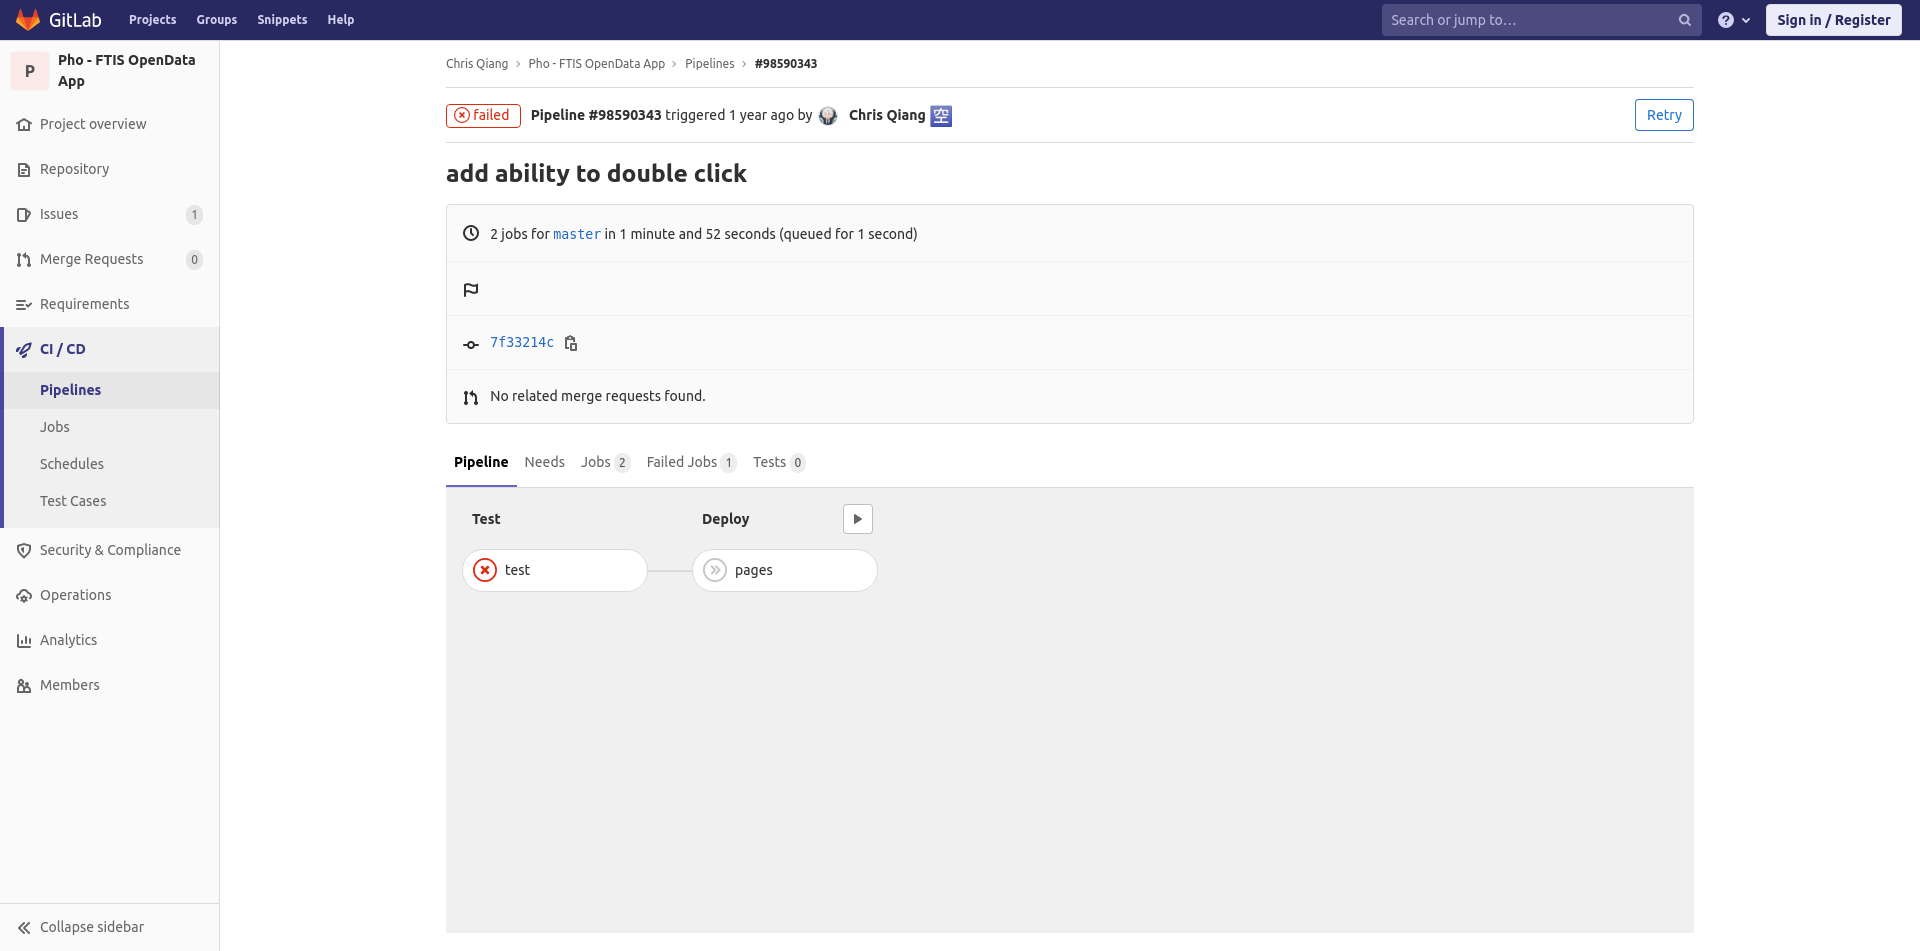
\includegraphics[width=0.7\paperwidth]{Gambar/gitlab-ci-job-view.png}
            \caption{Eksekusi \textit{job} yang gagal pada GitLab CI/CD.
            Repositori dari Pho - FTIS OpenData App\footnote{Lihat
            https://gitlab.com/chez14/ftis-opendata-app}}
            \label{fig:gitlab-ci:jobrun}
        \end{minipage}
    \end{figure}
    
    
    \textit{Script} yang ada akan dikelompokkan sebagai \textit{jobs}.
    Sekumpulan \textit{job} akan membentuk \textit{pipeline}.
    
    Sebagai contoh, berkas \texttt{.gitlab-ci.yml} memiliki format minimal
    sebagai berikut:
    
    \begin{verbatim}
    before_script:
      - apt-get install rubygems ruby-dev -y

    run-test:
      script:
        - ruby --version
    \end{verbatim}
    
    Pada berkas contoh, format \texttt{.gitlab-ci.yml} memiliki format YAML.
    Oleh karena itu indentasi denga spasi dan tabulasi akan sangat berpengaruh.
    Bagian pertama pada berkas tersebut adalah bagian \texttt{before\_script}.
    Pada bagian ini, perintah yang dilakukan adalah melakukan instalasi penjalan
    \textit{script} ruby, dan lingkungan pengembangannya.
    
    Berikutnya, sebuah \textit{job} dengan nama \texttt{run-test} akan
    ditambahkan pada sebuah \textit{pipeline} pada dasbor CI/CD pada GitLab.
    Lingkungan pada \texttt{before\_script} akan digunakan pada \textit{job} ini
    untuk melakukan eksekusi pada \textit{script} yang diberikan. Seperti pada
    contoh Gambar \ref{fig:gitlab-ci:jobrun}. Jika perintah tersebut gagal
    dieksekusi, maka \textit{job} pada tahap berikutnya tidak akan dieksekusi,
    dan pemilik kode akan diberitahu bahwa kompilasi gagal.
    
    
    \begin{figure}
        \begin{minipage}{\textwidth}
            \centering
            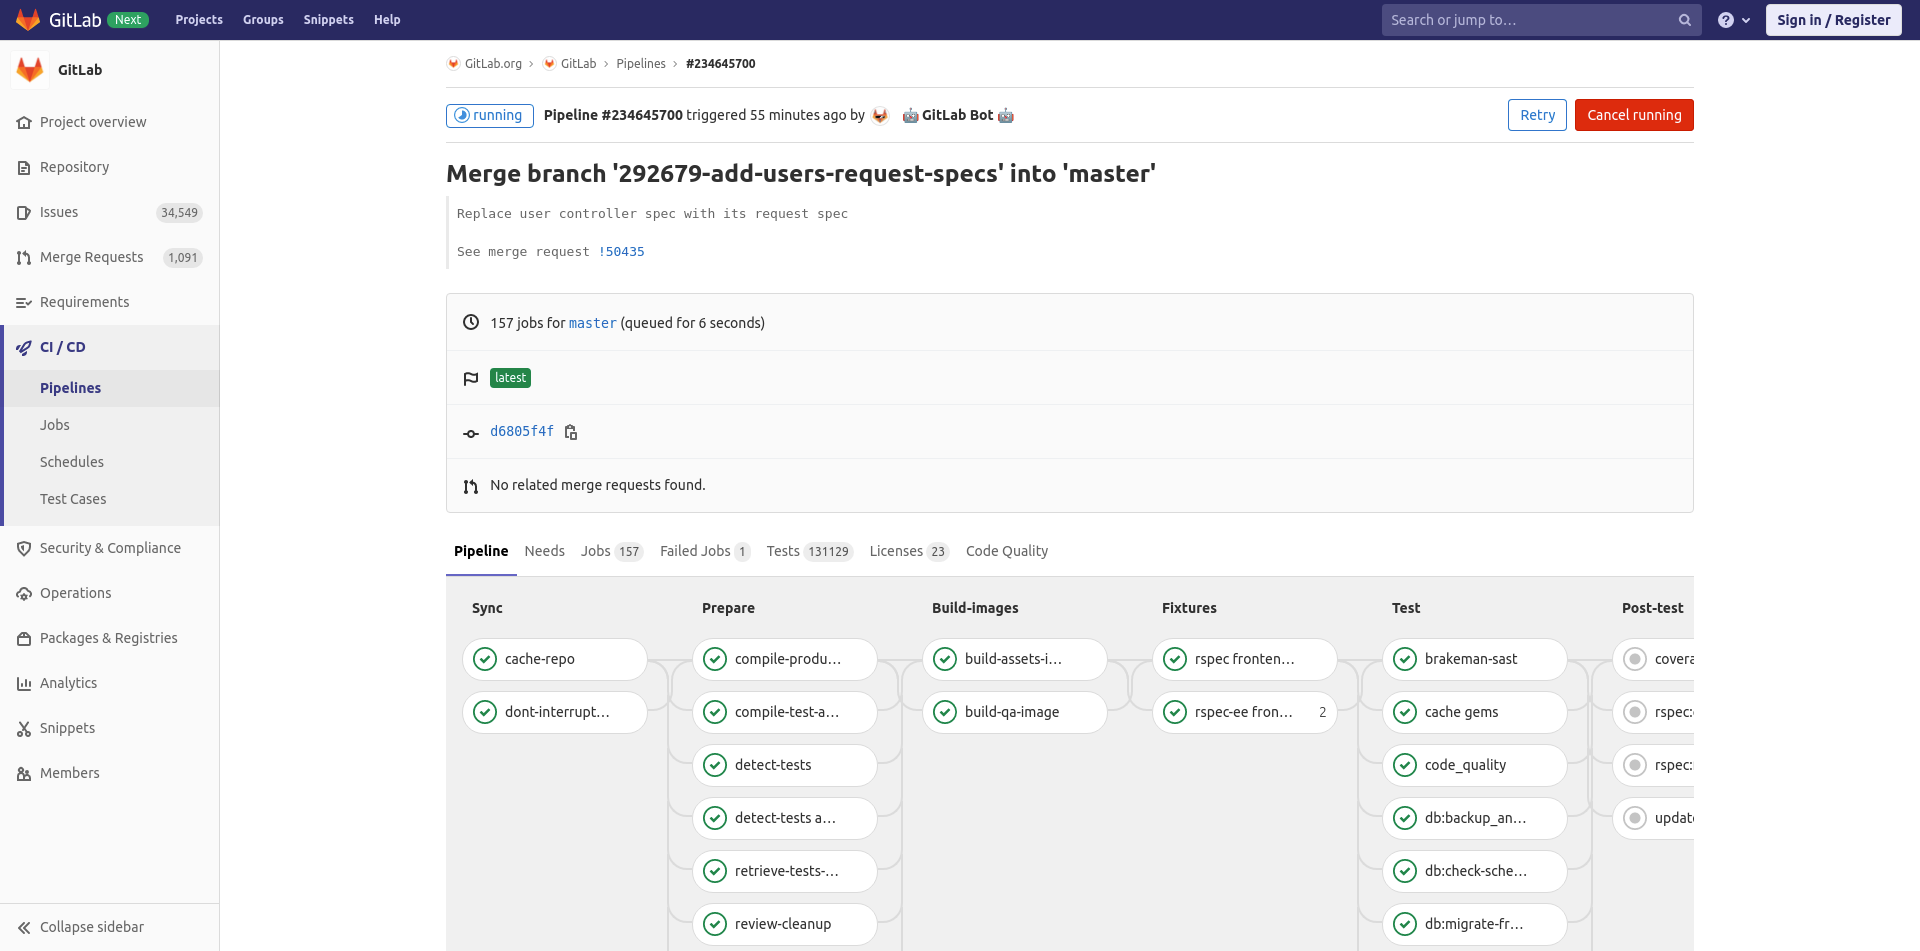
\includegraphics[width=0.7\paperwidth]{Gambar/gitlab-ci-pipeline.png}
            \caption{Contoh \textit{Pipeline} pada GitLab CI/CD. Repositori dari
            GitLab\footnote{Lihat https://gitlab.com/gitlab-org/gitlab}.}
            \label{fig:gitlab-ci:pipeline}
        \end{minipage}
    \end{figure}
    
    Dengan melakukan konfigurasi tertentu, pemilik proyek dapat membuat rencana
    CI/CD yang lebih kompleks dan bertahap. \textit{Pipeline} yang sudah dibuat
    akan ditampilkan pada dasbor secara diagram (Gambar
    \ref{fig:gitlab-ci:pipeline}).

\section{Docker}
    \textit{Containerization} adalah salah satu bentuk abstraksi pada level
    aplikasi yang membungkus kode dan kebutuhan \textit{dependenciy}-nya.
    Sehingga aplikasi berjalan secara konsisten pada berbagai sistem
    operasi\cite{docker:what-is-container}. Kontainer ini akan menjalankan
    \textit{image} yang memiliki kernel yang sama ataupun berbeda antar satu dan
    yang lain. Selain itu Kontainer juga mungkin dapat berbagi kernel antara
    satu \textit{image} dengan yang lain.
    
    Lingkungan produksi adalah lingkungan yang digunakan oleh server yang
    melayani permintaan kustomer. Karena lingkungan tersebut tempat aplikasi
    dijalankan, maka lingkungan pengembangan sebaik mungkin dibuat semirip
    mungkin dengan lingkungan produksi. Jika lingkungan produksi dapat
    dikontainerisasi, maka kita dapat menyalin kontainer tersebut dan membuatnya
    menjadi lingkungan pengembangan. Jika lingkungan pengembangan membutuhkan
    lingkungan produksi untuk diperbaharui, maka kontainer tersebut hanya perlu
    disalin ulang dan dijalankan kembali.
    
    \begin{figure}[H]
        \centering
        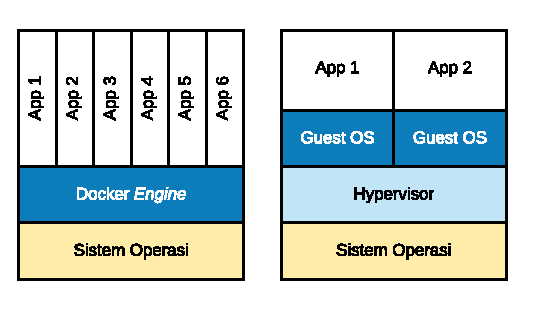
\includegraphics{Gambar/illust-docker.pdf}
        \caption{Ilustrasi perbandingan lapisan sistem pada Docker (kiri) dan
        \textit{Virtual Machine} (kanan)}
        \label{fig:illust-docker}
    \end{figure}
    
    Kontainer akan menjalankan \textit{image} diatas \textit{platform} mereka
    setelah infrastruktur operating sistem itu sendiri (Gambar
    \ref{fig:illust-docker} kiri). Berbeda dengan \textit{Virtual Machine} (atau
    VM), aplikasi pada kontainer tidak berjalan di atas sistem operasi yang
    dijalankan oleh VM (Gambar \ref{fig:illust-docker} kanan). \textit{Image}
    pada kontainer itu sendiri biasnaya berukuran cukup kecil (puluhan hingga
    ratusan MB), sehingga menjalankan kontainer jauh lebih ringan dibanding
    menjalankan VM.
    
    \textit{Hypervisor} adalah salah satu aplikasi yang memungkinkan menjalankan
    VM diatas sistem operasi. (Gambar \ref{fig:illust-docker} kanan).
    \textit{Virtual Machine} yang dibuat biasanya akan menjalankan kernel sistem
    operasi dan \textit{dependencies}-nya, sehingga memori yang dibutuhkan
    sangat banyak.
    
    Dengan karakteristik seperti itu, aplikasi yang dijalankan pada Docker
    memiliki beberapa keunggulan.
    \begin{itemize}
        \item Cepat dan \textit{Portable} \\
            Docker dapat dikofigurasi dengan membuatkan berkas konfigurasi
            khusus. Berkas konfigurasi tersebut akan memberikan informasi
            \textit{image} yang akan digunakan. Sehingga waktu yang diperlukan
            untuk melakukan konfigurasi pada server baru relatif cepat. Waktu
            konfigurasi secara mayoritas akan habis pada saat pendefinisian
            berkas konfigurasi Docker tersebut.
            
        \item Konsisten \\
            Dengan memanfaatkan \textit{image} dan \textit{engine} Docker,
            aplikasi akan berjalan pada \textit{platform} yang sama. Dengan
            karakteristik seperti itu, aplikasi yang didirikan secara teori akan
            dapat berjalan dengan konsisten pada berbagai sistem operasi.
            
        \item Aman \\
            Karakteristik Docker yang berjalan secara terisolasi dapat
            meningkatkan keamanan hingga standar
            industri\cite{docker:what-is-container} secara \textit{default}.
    \end{itemize}
    